%\addcontentsline{toc}{chapter}{Discriminators \& Sampling}\label{ch:Discriminators}
\chapter{Discriminators \& sampling}
\label{ch:Discriminators}

The role of the discriminator is to determine the error (frequency or phase), based on current an previous I \& Q samples. This is computed every second incoherent dump (8ms), because a pair of samples is required to compute frequency. 

The Discriminator for both the FLL and PLL loops comes from Kaplan, and can be found on pages (Insert pages here).


\tikzset{
block/.style = {draw, fill=white, rectangle, minimum height=3em, minimum width=3em},
tmp/.style  = {coordinate}, 
sum/.style= {draw, fill=white, circle, node distance=1cm},
input/.style = {coordinate},
output/.style= {coordinate},
pinstyle/.style = {pin edge={to-,thin,black}
}
}

\begin{figure}[!htb]
\centering
\begin{tikzpicture}[auto, node distance=2cm,>=latex']

%\draw[dotted](-3,0.25) node {Coherent samples};
%\draw[dotted](-3,-1.5) node {Incoherent integration};
%\draw[dotted](-3,-3.5) node {Frequencies};

    

\foreach \x in {0,...,31}{
    \draw [fill=orange] (0.5*\x,0) rectangle (0.5*\x+0.5,0.5);
}

\foreach \x in {0,...,7}{
    \draw [fill=blue] (2*\x,-1) rectangle (2*\x+2,-2);
}

\foreach \x in {0,...,3}{
    \draw [fill=teal] (4*\x,-3) rectangle (4*\x+4,-4);
}

\foreach \x in {0,...,7}{
\draw [decorate,decoration={brace,amplitude=0.4cm,mirror},xshift=0,yshift=0pt]
(2*\x,0) -- (2*\x+2,0) node [black,midway]{};
}

\foreach \x in {0,...,7}{
    \draw[->] (2*\x+1,-0.4) -- (2*\x+1,-1);
}

\foreach \x in {0,...,3}{
    \draw [decorate,decoration={brace,amplitude=0.4cm,mirror},xshift=0,yshift=0pt]
(4*\x,-2) -- (4*\x+4,-2) node [black,midway]{};
}

\foreach \x in {0,...,3}{
    \draw[->] (4*\x+2,-2.4) -- (4*\x+2,-3);
}

\end{tikzpicture}
\caption{An overview of the sampling process.1 ms long coherently integrated samples (orange)  are produced by the hardware correlator.Four of these are coherently integrated together to generate the inputs to the tracking loop (blue). The FLL and PLL discriminator both take a pair of 4ms long samples to produce an estimate of the phase/frequency (teal).}
\label{fig:SamplingSchemeA}
\end{figure}






\tikzset{
block/.style = {draw, fill=white, rectangle, minimum height=3em, minimum width=3em},
tmp/.style  = {coordinate}, 
sum/.style= {draw, fill=white, circle, node distance=1cm},
input/.style = {coordinate},
output/.style= {coordinate},
pinstyle/.style = {pin edge={to-,thin,black}
}
}

\begin{figure}[!htb]
\centering
\begin{tikzpicture}[auto, node distance=2cm,>=latex']

%\draw[dotted](-3,0.25) node {Coherent samples};
%\draw[dotted](-3,-1.5) node {Incoherent integration};
%\draw[dotted](-3,-3.5) node {Frequencies};

\foreach \x in {0,...,31}{
    \draw [fill=orange] (0.5*\x,0) rectangle (0.5*\x+0.5,0.5);
}

\foreach \x in {0,...,7}{
    \draw [fill=blue] (2*\x,-1) rectangle (2*\x+2,-2);
}


\foreach \x in {0,...,7}{
    \draw [fill=teal] (2*\x,-3) rectangle (2*\x+2,-4);
}


\foreach \x in {0,...,7}{
    \draw [decorate,decoration={brace,amplitude=0.4cm,mirror},xshift=0,yshift=0pt]
(2*\x,0) -- (2*\x+2,0) node [black,midway]{};
    \draw[->] (2*\x+1,-0.4) -- (2*\x+1,-1);
}


\foreach \x in {0,...,3}{
    \draw [decorate,decoration={brace,amplitude=0.5cm,mirror},xshift=0,yshift=0pt]
(4*\x,-2) -- (4*\x+4,-2) node [black,midway]{};
    \draw[->] (4*\x+2,-2.5) -- (4*\x+1,-3);
}

\foreach \x in {0,...,2}{
    \draw [red,decorate,decoration={brace,amplitude=0.3cm,mirror},xshift=0,yshift=0pt]
(4*\x+2,-2) -- (4*\x+6,-2) node [black,midway]{};
    \draw[->,red] (4*\x+4,-2.3) -- (4*\x+3,-3);
}

\end{tikzpicture}
\caption{As compared to the sampling process outlined in figure \ref{fig:SamplingSchemeA}, this scheme provides frequency and phase estimates every 4ms.}
\label{fig:SamplingB}
\end{figure}






\tikzset{
block/.style = {draw, fill=white, rectangle, minimum height=3em, minimum width=3em},
tmp/.style  = {coordinate}, 
sum/.style= {draw, fill=white, circle, node distance=1cm},
input/.style = {coordinate},
output/.style= {coordinate},
pinstyle/.style = {pin edge={to-,thin,black}
}
}

\begin{figure}[!htb]
\centering
\begin{tikzpicture}[auto, node distance=2cm,>=latex']

%\draw[dotted](-3,0.25) node {Coherent samples};
%\draw[dotted](-3,-1.5) node {Incoherent integration};
%\draw[dotted](-3,-3.5) node {Frequencies};


\draw[->] (1,1) -- (1,0.5);
\draw[->] (3,1) -- (3,0.5);
\node at (1,1.2) {$\phi_1$};
\node at (3,1.2) {$\phi_2$};


\foreach \x in {0,...,7}{
    \draw [fill=orange] (0.5*\x,0) rectangle (0.5*\x+0.5,0.5);
}


\foreach \x in {0,...,7}{
    \draw [fill=orange] (0.5*\x+9,0) rectangle (0.5*\x+0.5+9,0.5);
}


\node at (4.5,0) {\ldots};


\foreach \x in {0,...,1}{
    \draw [fill=blue] (2*\x,-1) rectangle (2*\x+2,-2);
}

\draw [fill=teal] (0,-3) rectangle (4,-4);


\foreach \x in {0,...,1}{
    \draw [decorate,decoration={brace,amplitude=0.4cm,mirror},xshift=0,yshift=0pt]
(2*\x,0) -- (2*\x+2,0) node [black,midway]{};
    \draw[->] (2*\x+1,-0.4) -- (2*\x+1,-1);
}


\draw [decorate,decoration={brace,amplitude=0.5cm,mirror},xshift=0,yshift=0pt]
(0,-2) -- (4,-2) node [black,midway]{};
\draw[->] (2,-2.5) -- (2,-3);


\draw[->] (4,-4) -- (4,-5);
\draw [fill=purple] (4,-5) rectangle (5.5,-6);
\node at (4.75,-5.5) {Jitter};


\draw[->] (5.5,-6) -- (5.5,-7);
\draw [fill=yellow] (5.5,-7) rectangle (7.5,-8);
\node at (6.5,-7.25) {Tracking};
\node at (6.5,-7.75) {Loop};


\draw[->] (7.5,-8) -- (7.5,-9);
\draw [fill=purple] (7.5,-9) rectangle (9,-10);
\node at (8.25,-9.5) {Jitter};

\draw[->] (9,-9) -- (9,0);
\node at (10.5,-0.5) {Update NCO};


\draw [decorate,decoration={brace,amplitude=0.4cm},xshift=0,yshift=0pt]
(3,0.5) -- (9,0.5) node [black,midway]{};

%\draw[->] (9,1.5) -- (9,0.5);
\node at (6,1.2) {Delay};


\end{tikzpicture}
\caption{Once a pair of 4ms coherently integrated samples has been collected, then the tracking loops can compute a new value for the NCO. During this process, delays accrue due to the interrupt driven nature of the processor, as well as processing time for the tracking loops.}
\label{fig:SamplingJitter}
\end{figure}






\begin{comment}
"It is important to note that the timing of each of the correlator channels will be locked to its own incoming signal and not to each other or to the microprocessor interrupts, so new data is generated asynchronously. The sampling instant of measurement data of all channels however is common to give a consistent navigation solution."

"Carrier DCO Programming
The following registers: CHx_CARRIER_DCO_INCR_HIGH (or X_DCO _INCR_HIGH) and CHx_CARRIER_DCO_INCR_LOW
are programmed in sequence with the relevant data according to the frequency bin being searched. It is always necessary to write to both the _HIGH and _LOW registers. Carrier DCO programming will become effective as soon as the channel is released (made active). If the channel is already active, writes to CHx_CARRIER_DCO_INCR_LOW are effective immediately. (A short delay of up to 175ns will occur, to allow synchronisation of the processor write operation to the chip operation.)"
\cite{GP2021}
\end{comment}

\subsection{Arctangent}
The arctangent function is used in the discriminators for both the FLL and the PLL. It is important to note that there are two different types of arctangent function, the 
\lstinputlisting[language=Python,frame=single]{Code/ATan2.py}

Some additional logic is included in the function to ensure that the function always returns a value, even when X is equal to zero.

\begin{figure}[!htb] 
    \centering
    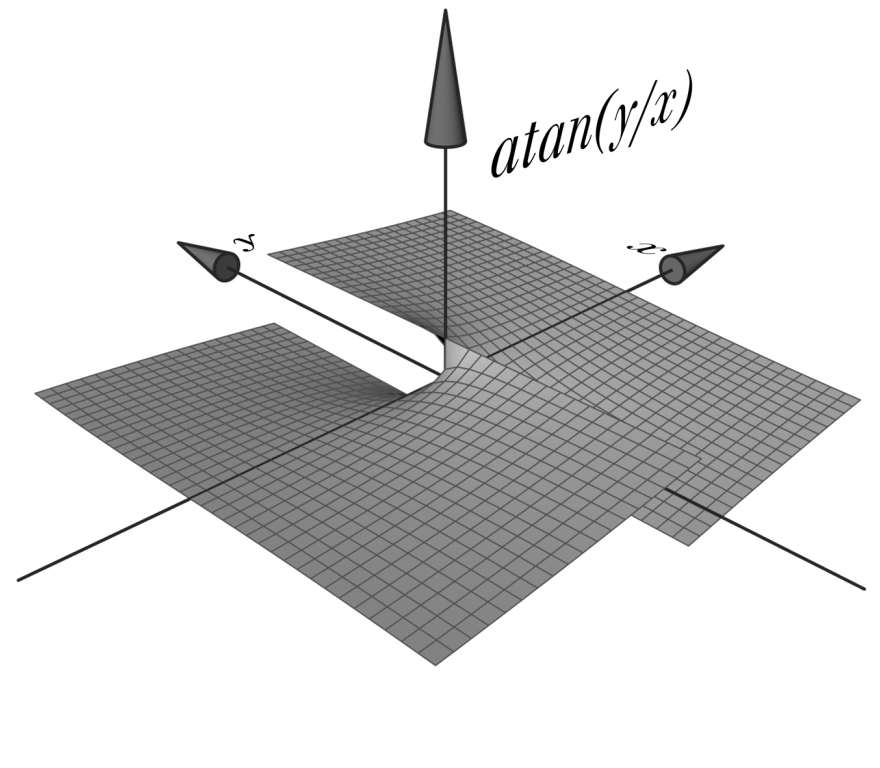
\includegraphics[width=1\textwidth]{Discriminators/ATanDiagram.png} 
    \caption{}
    \label{fig:ATanDiagram}
\end{figure}

\begin{figure}[!htb] 
    \centering
    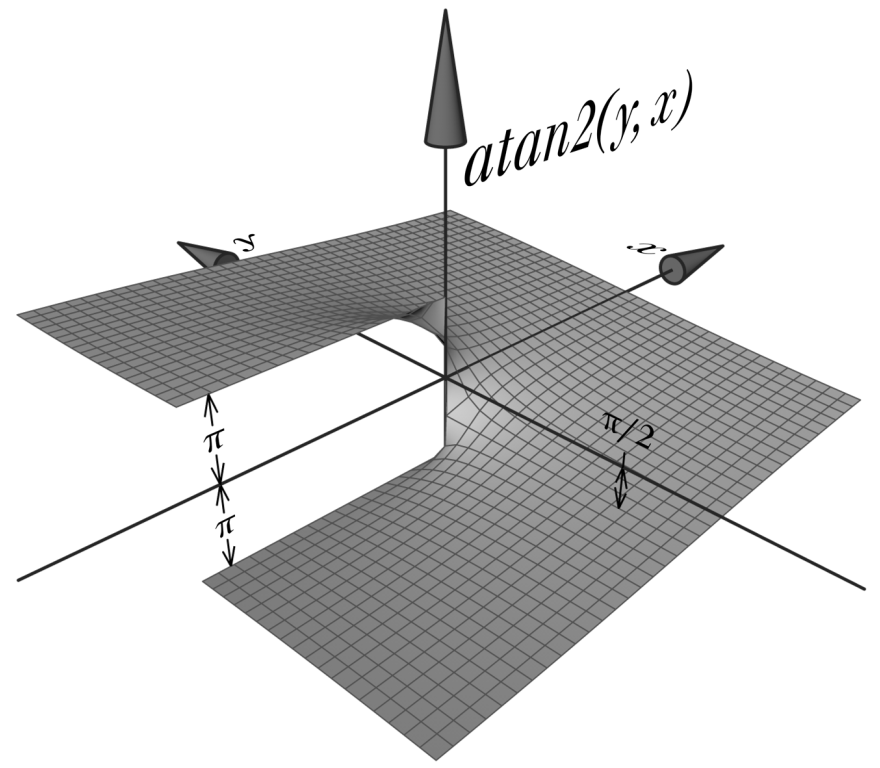
\includegraphics[width=1\textwidth]{Discriminators/ATan2Diagram.png} 
    \caption{}
    \label{fig:ATan2Diagram}
\end{figure}


\subsection{FLL discriminator}
The role of the FLL discriminator is to convert pairs of phase measurements into frequency. A key statistic for the FLL discriminator is it's capture range. This can be computed as 
$\frac{-1}{2T} < f < \frac{1}{2T}$
, where $T = 0.004S$

Hence the FLL has a locking range of $\pm 125Hz$. 

If the frequency of the incoming signal is outside this range, then a false lock will occur due to aliasing. This can be seen in figure(Insert picture of aliasing). 

The FLL discriminator which is described in Kaplan uses the dot and cross product of the previous two samples.

\begin{align*}
\text{Dot} &= I_{k}\times I_{k-1} + Q_{k}\times Q_{k-1}\\
\text{Cross} &= Q_{k} \times I_{k-1} - I_{k} \times K_{k-1}\\
\text{DeltaPhase} &= ATan2(Cross,Dot)
\end{align*}


\begin{figure}[!htb] 
    \centering
    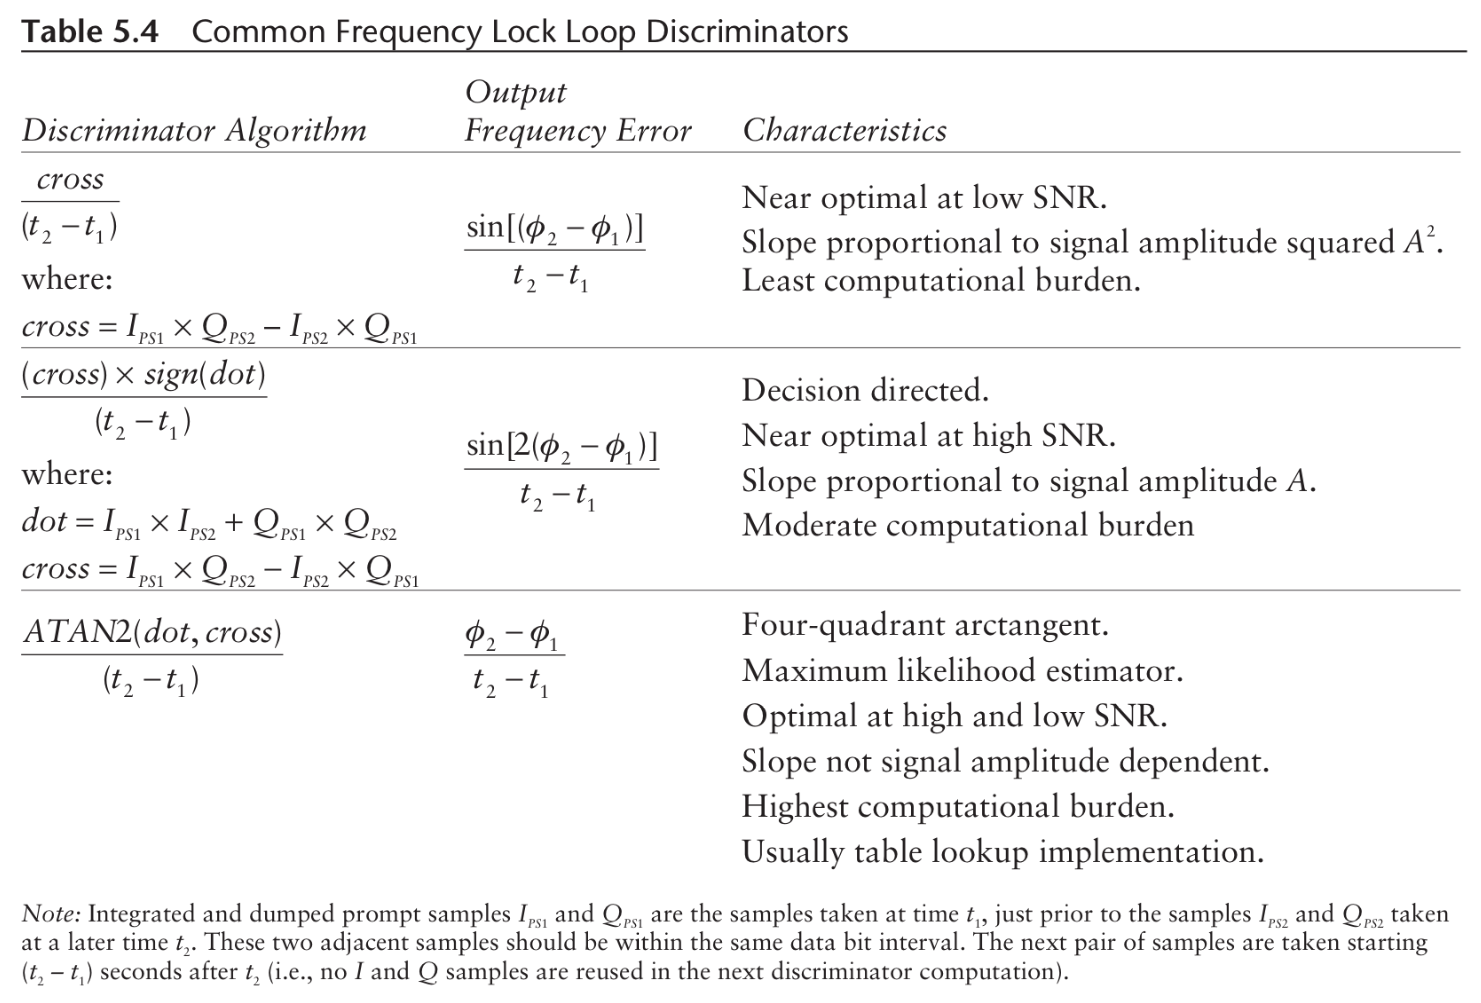
\includegraphics[width=1\textwidth]{Discriminators/FLLDiscriminator.png} 
    \caption{The different FLL discriminators presented in Kaplan.\cite{Kaplan}}
    \label{fig:FLLDiscriminatorTable}
\end{figure}


\lstinputlisting[language=Python,frame=single]{Code/FLLDiscriminator.py}

\subsection{PLL discriminator}
The goal of the PLL Discriminator is to determine the current phase error. In the case of the current implementation, computed phase 


\begin{figure}[!htb] 
    \centering
    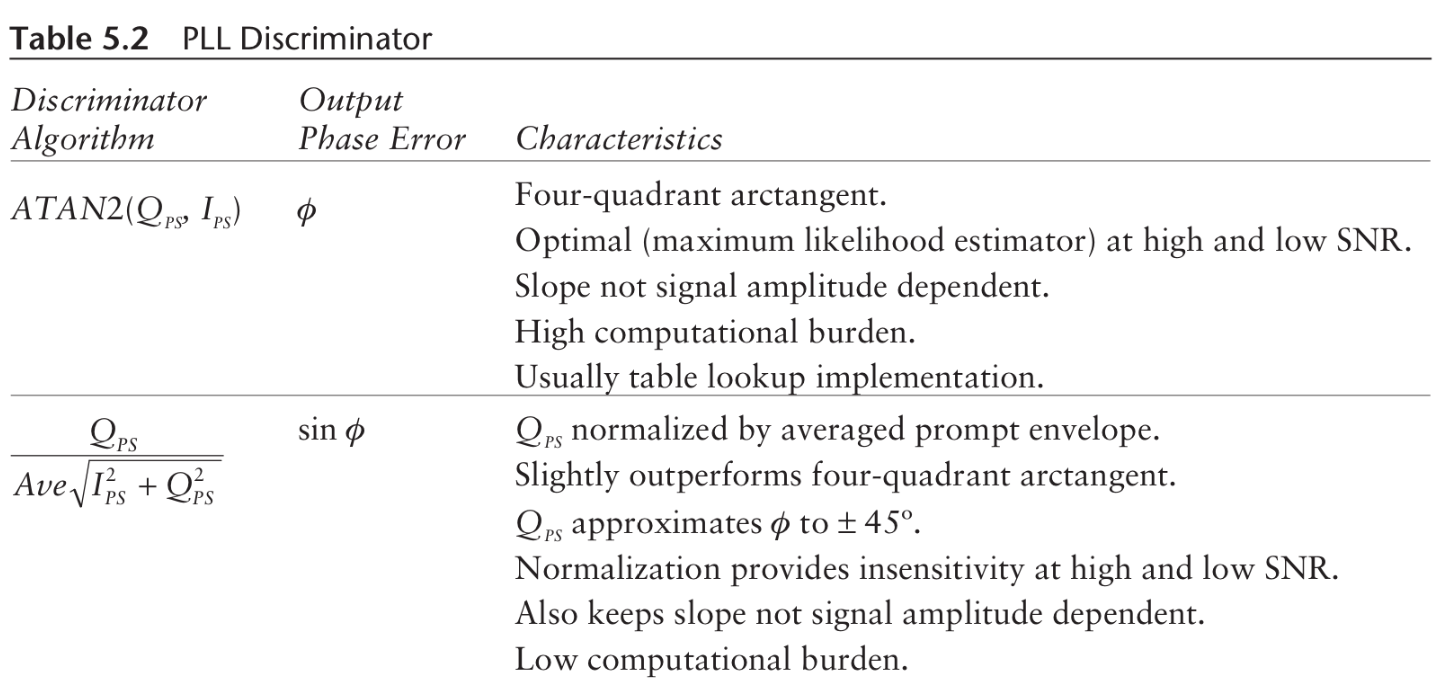
\includegraphics[width=1\textwidth]{Discriminators/PLLDiscriminator.png} 
    \caption{The different PLL discriminators presented in Kaplan.\cite{Kaplan}}
    \label{fig:PLLDiscriminatorTable}
\end{figure}

\begin{figure}[!htb] 
    \centering
    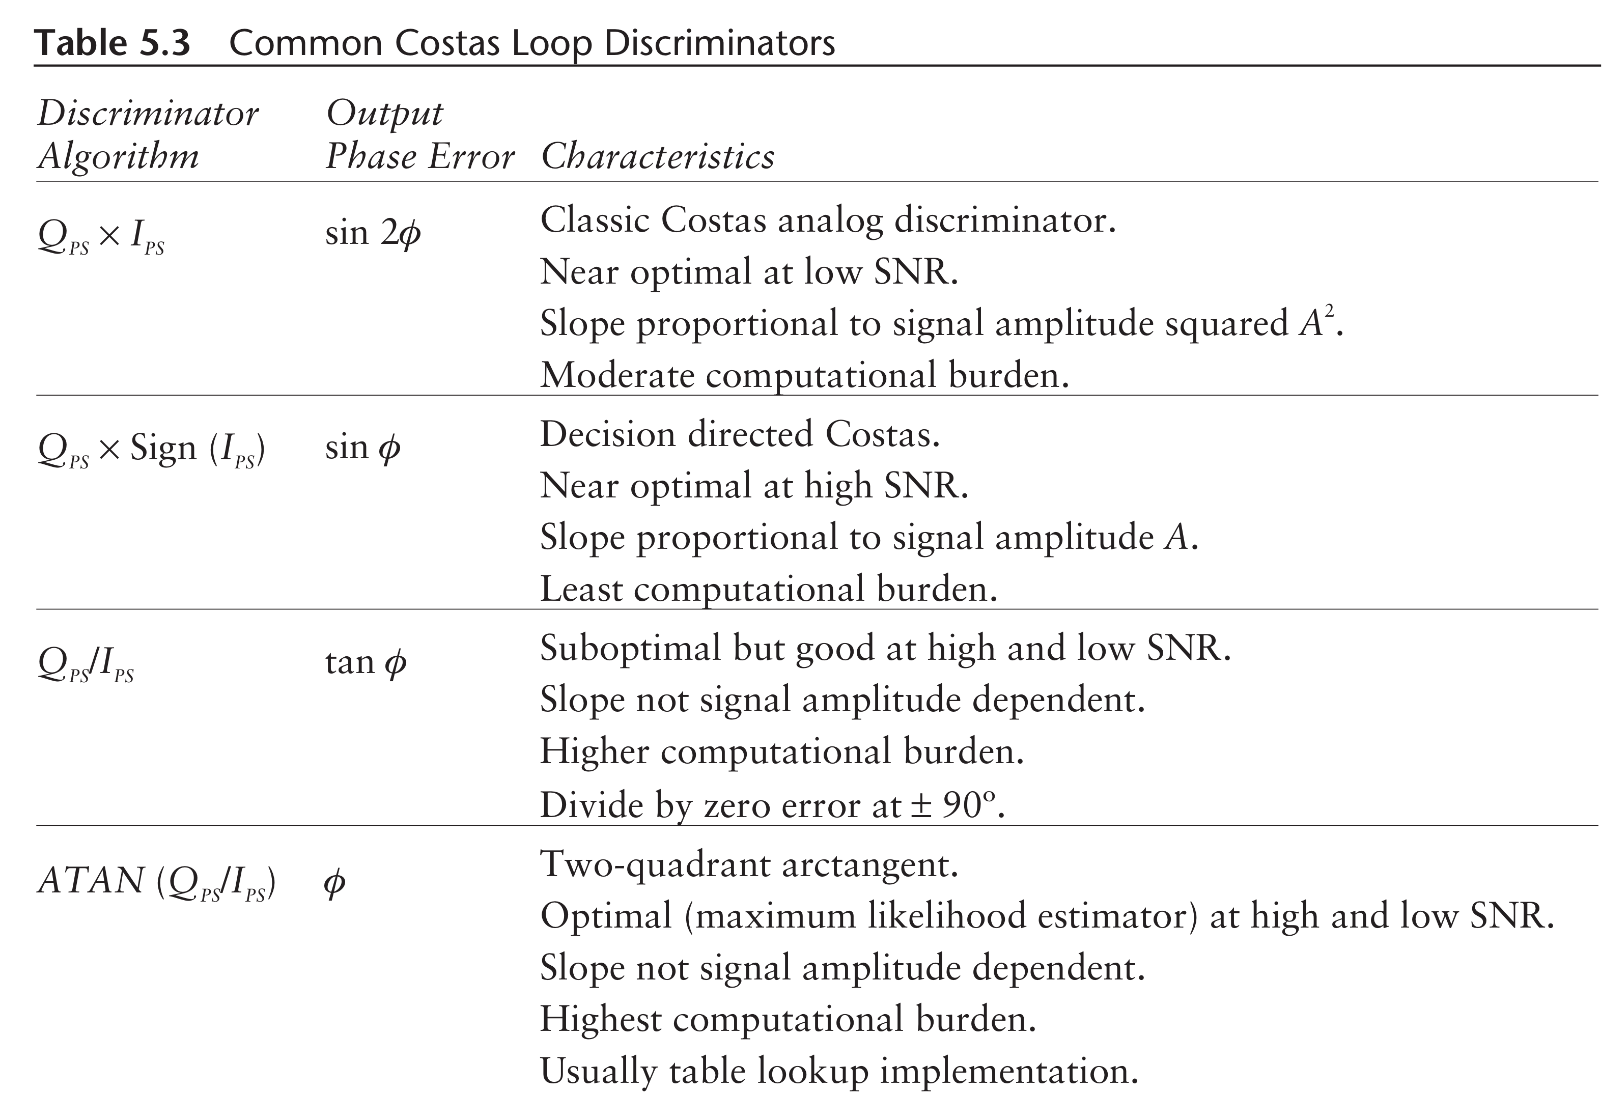
\includegraphics[width=1\textwidth]{Discriminators/CostasDiscriminator.png} 
    \caption{The different Costas loop discriminators presented in Kaplan.\cite{Kaplan}}
    \label{fig:CostasDiscriminatorTable}
\end{figure}

$Z_{k} \times \overline{Z_{k-1}}$

%\lstinputlisting[language=Python,frame=single]{Code/PLLDiscriminator.py}
